\documentclass[12pt,a4paper]{report}
\usepackage[utf8]{inputenc}
\usepackage{amsmath}
\usepackage{graphicx}
\usepackage{booktabs}
\usepackage[hidelinks]{hyperref}
\usepackage{geometry}
\geometry{a4paper, margin=1in}
\usepackage{titlesec}
\usepackage{tikz}
\usetikzlibrary{shapes.geometric, arrows.meta, positioning, calc, fit, backgrounds}
\usepackage{setspace}
\usepackage{float}
\usepackage{subcaption}

\onehalfspacing

\begin{document}

\begin{titlepage}
    \centering
    \vspace*{2cm}
    
    {\Huge \textbf{Multi-Task Temporal Transformer for Ship Motion and Propeller Operability Prediction} \par}
    
    \vspace{2cm}
    {\Large \textit{B.Tech Project Report} \par}
    
    \vspace{1.5cm}
    {\normalsize By \par}
    \vspace{0.5cm}
    {\Large \textbf{Kush Chaudhari} \par}
    {\large 22NA3AI39 \par}
    
    \vspace{2cm}
    {\normalsize Under the Guidance of \par}
    \vspace{0.5cm}
    {\Large \textbf{Prof. Hari Warrior} \par}
    
    \vfill
    
    {\large \today \par}
\end{titlepage}

\begin{abstract}
Predicting the seakeeping behavior of a vessel is crucial for ensuring operational safety, passenger comfort, and structural integrity. Recently, deep learning surrogate models have emerged as computationally efficient alternatives to traditional hydrodynamic solvers. In the previous phase of this project, a Transformer-based model was successfully developed to predict the 6-Degrees of Freedom (6-DoF) ship motions from simulated time-series data. In this phase, the simulation environment was augmented by introducing a propeller disc representation at the stern of the vessel. This report details the development of a Multi-Task Temporal Transformer designed not only to forecast the 6-DoF motions but also to simultaneously predict propeller operability. Specifically, the model continuously estimates a Propeller Emergence Score and classifies binary emergence events to prevent ventilation and efficiency losses. By evaluating the model under different emergence thresholds, we demonstrate near-perfect motion regression ($R^2 > 0.999$) and highly accurate emergence classification (F1-Score $> 0.99$), proving the viability of multi-task Transformers in complex maritime forecasting applications.
\end{abstract}

\tableofcontents
\listoffigures
\listoftables

\chapter{Introduction}
\section{Background and Motivation}
The behavior of a ship navigating through rough seas is governed by complex, non-linear hydrodynamic interactions. Predicting these motions—specifically the 6-Degrees of Freedom (6-DoF): surge, sway, heave, roll, pitch, and yaw—is a fundamental component of maritime engineering. Traditional approaches rely on Potential Flow theory or Computational Fluid Dynamics (CFD). While accurate, these solvers are computationally expensive and cannot be deployed for real-time, on-board predictive decision-making. 

In recent years, data-driven approaches, particularly deep learning models like Long Short-Term Memory (LSTM) networks and Transformers, have shown immense promise as surrogate models. In the preceding semester, a temporal Transformer architecture was validated for 6-DoF motion prediction, establishing that self-attention mechanisms are highly capable of capturing the underlying wave-structure interactions.

\section{Problem Statement: Propeller Operability}
While predicting the hull's motion is critical, the operational efficiency of the vessel is heavily dictated by its propulsion system. In rough seas, excessive pitch and heave can cause the stern of the ship to rise significantly, leading to \textit{propeller emergence} (or ventilation). When the propeller blades break the water surface, several detrimental effects occur:
\begin{itemize}
    \item \textbf{Loss of Thrust:} Air is drawn into the propeller disc, drastically reducing the thrust and overall propulsion efficiency.
    \item \textbf{Vibrations and Structural Fatigue:} The sudden change in hydrodynamic loading causes severe vibrations, accelerating mechanical wear on the propeller shaft and bearings.
    \item \textbf{Engine Over-speeding:} A sudden loss of resistance can cause the main engine to over-speed, potentially triggering automatic shutdowns.
\end{itemize}

\section{Objectives of Phase 2}
The primary objective of this phase is to extend the existing Transformer surrogate model to not only predict the 6-DoF motions but to explicitly monitor and predict the state of the propeller. The specific goals are:
\begin{enumerate}
    \item Incorporate a geometric representation of the propeller (a disc) into the Maxsurf simulation environment to extract local stern responses.
    \item Formulate a continuous mathematical metric (Emergence Score) and a discrete metric (Emergence Flag) to quantify propeller ventilation.
    \item Design and train a Multi-Task Temporal Transformer capable of simultaneously performing multi-variate regression (for motions and the continuous score) and binary classification (for the emergence flag).
    \item Evaluate the model's performance under varying operational thresholds to prove its robustness as an early-warning predictive system for ship routing.
\end{enumerate}


\chapter{Data Generation and Simulation}
\section{Vessel Specifications}
The simulation vessel is a full-load container ship representative of modern ultra-large container vessels (ULCVs). Generating accurate time-series data requires a highly defined hull geometry to properly calculate the hydrodynamic coupling across all degrees of freedom. Its principal particulars are summarized in Table \ref{tab:vessel_specs}.

\begin{table}[H]
\centering
\caption{Vessel Specifications}
\label{tab:vessel_specs}
\vspace{0.2cm}
\begin{tabular}{@{}ll@{}}
\toprule
\textbf{Parameter} & \textbf{Value} \\ \midrule
Vessel Type & Container Vessel \\
Length Overall (LOA) & $\sim 350$ m \\
Draft (Full Load) & 15 m \\
Vessel Speeds Simulated & 2, 5, 8 knots \\
Simulation Software & Maxsurf Motions (MOSES Strip Theory) \\ \bottomrule
\end{tabular}
\end{table}

\section{Simulation Setup}
Time-domain simulations were conducted in irregular waves characterized by the JONSWAP (Joint North Sea Wave Project) energy spectrum, which is widely used for modelling wind-generated ocean waves in design and operational scenarios. Simulations were performed at three forward speeds—2, 5, and 8 knots—to capture the effect of vessel speed on hydrodynamic coupling. For each speed, the vessel's six-component motion response (surge, sway, heave, roll, pitch, yaw) was recorded at a nominal sampling rate, subsequently processed to a uniform 10 Hz grid. The simulation parameters are summarized in Table \ref{tab:sim_params}.

\begin{table}[H]
\centering
\caption{Simulation Parameters}
\label{tab:sim_params}
\vspace{0.2cm}
\begin{tabular}{@{}ll@{}}
\toprule
\textbf{Parameter} & \textbf{Value} \\ \midrule
Wave Spectrum & JONSWAP \\
Wave Type & Irregular (Random Seas) \\
Vessel Speeds & 2 kn, 5 kn, 8 kn \\
Output Sampling Rate & 10 Hz (uniform grid) \\
Degrees of Freedom & 6 (Surge, Sway, Heave, Roll, Pitch, Yaw) \\ \bottomrule
\end{tabular}
\end{table}

\subsection{Integrating the Propeller Disc}
Instead of modeling the complex hydrodynamics of the rotating propeller blades within the seakeeping solver, a geometrical reference point was established. A \texttt{PROP\_REF\_DISC} was added to the Maxsurf Modeler at the stern of the vessel. The coordinates of the propeller center and the propeller diameter were recorded. This approach ensures that the fundamental hull hydrostatics remain unchanged, while allowing Maxsurf Motions to compute the exact kinematic response at the specific location of the propeller disc. Figure \ref{fig:sim_pipeline} illustrates the complete data generation workflow.

\begin{figure}[H]
    \centering
    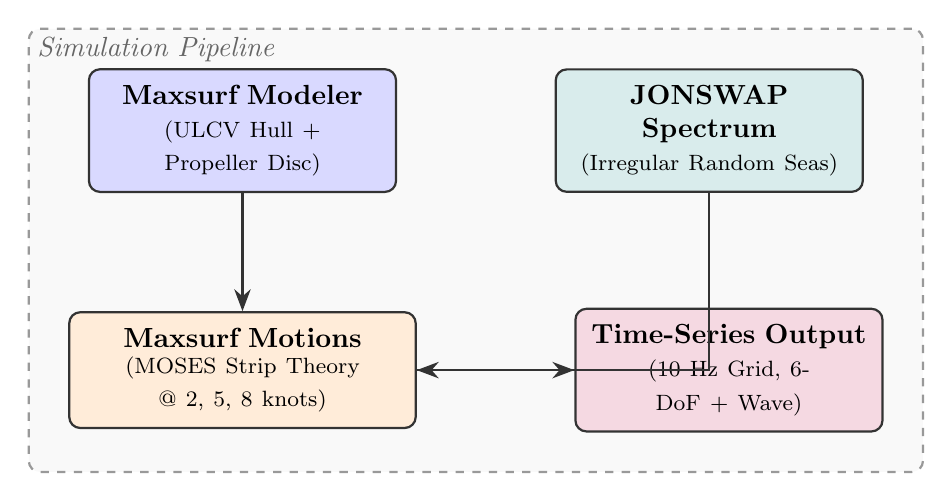
\begin{tikzpicture}[
        node distance=1.5cm and 2cm,
        box/.style={rectangle, draw=black!80, thick, fill=blue!15, text width=3.5cm, align=center, rounded corners, minimum height=1.2cm, inner sep=0.2cm},
        env/.style={rectangle, draw=black!80, thick, fill=teal!15, text width=3.5cm, align=center, rounded corners, minimum height=1.2cm, inner sep=0.2cm},
        process/.style={rectangle, draw=black!80, thick, fill=orange!15, text width=4cm, align=center, rounded corners, minimum height=1.2cm, inner sep=0.2cm},
        output/.style={rectangle, draw=black!80, thick, fill=purple!15, text width=3.5cm, align=center, rounded corners, minimum height=1.2cm, inner sep=0.2cm},
        arrow/.style={-{Stealth[scale=1.2]}, thick, color=black!80}
    ]
    
    % Nodes
    \node[box] (modeler) {\textbf{Maxsurf Modeler}\\ \footnotesize (ULCV Hull + Propeller Disc)};
    \node[env] (wave) [right=2cm of modeler] {\textbf{JONSWAP Spectrum}\\ \footnotesize (Irregular Random Seas)};
    \node[process] (motions) [below=1.5cm of modeler] {\textbf{Maxsurf Motions}\\ \footnotesize (MOSES Strip Theory \\ @ 2, 5, 8 knots)};
    \node[output] (csv) [right=2cm of motions] {\textbf{Time-Series Output}\\ \footnotesize (10 Hz Grid, 6-DoF + Wave)};
    
    % Grouping Box
    \begin{scope}[on background layer]
        \node[draw=black!40, dashed, thick, rounded corners, fill=gray!5, inner sep=0.5cm, fit=(modeler) (wave) (motions) (csv)] (pipeline) {};
        \node[anchor=north west, color=black!60, font=\itshape] at (pipeline.north west) {Simulation Pipeline};
    \end{scope}

    % Connections
    \draw[arrow] (modeler) -- (motions);
    \draw[arrow] (wave.south) |- (motions.east);
    \draw[arrow] (motions) -- (csv);
    
    \end{tikzpicture}
    \caption{Data Generation Pipeline: From geometric hull modelling and JONSWAP wave generation to the final 10 Hz multivariate time-series extraction.}
    \label{fig:sim_pipeline}
\end{figure}

\section{Formulating the Propeller Emergence Metrics}
While Maxsurf outputs the raw motions, the actual analysis of propeller emergence is performed downstream during data preprocessing. Because the propeller is located at the stern, the vertical motion of the propeller center is strongly correlated with the ship's global heave and pitch. For this study, the global heave amplitude is utilized as a proxy for the vertical displacement at the stern.

We define the \textbf{Emergence Score ($E$)} as the ratio of the upward motion amplitude to the static depth of the propeller:
\begin{equation}
    E = \frac{A_{\text{upward at prop center}}}{h_{\text{top, static}}} \approx \frac{|\text{Heave Amplitude}|}{h_{\text{static}}}
\end{equation}
Where $h_{\text{static}}$ is the depth of the top of the propeller disc below the calm waterline. 

From this continuous score, a binary \textbf{Emergence Flag} is derived to classify the ventilation event:
\begin{equation}
    \text{Flag} = 
    \begin{cases} 
      1 & \text{if } E \geq 1.0 \\
      0 & \text{if } E < 1.0
    \end{cases}
\end{equation}

By extracting these values, the dataset is transformed into a multi-target format suitable for training the deep learning model.

\subsection{Dataset Statistics}
The generated dataset comprises 6,733 raw timesteps. To understand the operational conditions simulated, Table \ref{tab:dataset_stats} presents the descriptive statistics for the wave elevation and the corresponding 6-DoF responses. The maximum wave amplitude observed was approximately $\pm 4.18m$, which induced a maximum heave displacement of $\pm 2.88m$ and pitch variations up to $\pm 2.47^\circ$. The standard deviations indicate a highly dynamic sea state, providing a robust distribution for training the predictive models.

\begin{table}[H]
\centering
\caption{Descriptive Statistics of the Simulated Maxsurf Dataset (6,733 samples)}
\label{tab:dataset_stats}
\vspace{0.2cm}
\begin{tabular}{@{}lcccc@{}}
\toprule
\textbf{Variable} & \textbf{Minimum} & \textbf{Maximum} & \textbf{Mean} & \textbf{Std. Dev.} \\ \midrule
Wave ($m$) & -4.183 & +4.183 & 0.014 & 2.962 \\
Surge ($m$) & -1.369 & +1.369 & -0.003 & 0.966 \\
Sway ($m$) & -1.327 & +1.327 & -0.004 & 0.938 \\
Heave ($m$) & -2.883 & +2.883 & 0.009 & 2.040 \\
Roll ($deg$) & -0.320 & +0.320 & 0.001 & 0.226 \\
Pitch ($deg$) & -2.474 & +2.474 & 0.005 & 1.746 \\
Yaw ($deg$) & -1.049 & +1.049 & -0.003 & 0.742 \\ \bottomrule
\end{tabular}
\end{table}

\section{Feature Correlation Analysis}
To ensure the machine learning model focuses on physically meaningful relationships rather than noise, a preliminary correlation analysis was conducted. It was observed that the calculated Emergence Score ($E$) exhibits a strong positive correlation with the global heave and pitch signals. This aligns with fundamental seakeeping theory: large vertical displacements and rotational pitching directly dictate the vertical trajectory of the stern propeller disc. The Transformer architecture is inherently well-suited to capture these multivariate correlations across the 10-second input temporal window.

\begin{figure}[H]
    \centering
    \includegraphics[width=0.85\textwidth]{figures/correlation_heatmap.png}
    \caption{Pearson correlation heatmap demonstrating the physical dependencies between the wave excitation, 6-DoF responses, and the derived Propeller Emergence Score.}
    \label{fig:corr_heatmap}
\end{figure}


\chapter{Methodology}
\section{Data Preprocessing}
Before feeding the data into the deep learning model, a robust preprocessing pipeline was established to handle the temporal complexities of the simulation output.

\subsection{Temporal Interpolation and Normalization}
The raw Maxsurf output contained non-uniform timesteps. To establish a consistent temporal grid required for sequence modeling, cubic spline interpolation was applied to resample all signals (wave and 6-DoF motions) to a uniform 10 Hz frequency. Following interpolation, the features were scaled using standard $Z$-score normalization to ensure the network gradients remain stable during backpropagation.

\subsection{Feature Engineering and Sequence Generation}
The continuous Emergence Score ($E$) was calculated by taking the rolling amplitude of the heave signal over a 0.5-second window. The binary Emergence Flag was subsequently derived. The time-series was then segmented into overlapping sliding windows. The input sequence consisted of 100 timesteps ($10$ seconds), and the target output sequence consisted of 50 timesteps ($5$ seconds) into the future. A temporal split was utilized for the dataset, allocating the final 20\% of the temporal sequence strictly for testing to prevent data leakage.

\section{Multi-Task Transformer Architecture}
The predictive engine is built upon the Transformer encoder architecture. Unlike traditional sequence models (e.g., LSTMs), Transformers utilize self-attention mechanisms, allowing them to capture long-range dependencies and complex phase relationships between the wave input and the ship's physical response.

\subsection{Network Design}
The architecture features a \textbf{Shared Encoder} backbone that processes the 7-dimensional input sequence. This sequence is first projected into a higher-dimensional embedding space ($d_{model} = 128$). Because Transformers lack inherent sequential inductive bias, \textbf{Positional Encodings} are injected to preserve temporal ordering. The encodings are mathematically formulated as:
\begin{align}
    PE_{(pos, 2i)} &= \sin\left(\frac{pos}{10000^{2i/d_{model}}}\right) \\
    PE_{(pos, 2i+1)} &= \cos\left(\frac{pos}{10000^{2i/d_{model}}}\right)
\end{align}
where $pos$ is the temporal position in the sequence and $i$ is the feature dimension index. This periodic encoding ensures the network can smoothly interpolate relative temporal distances between wave impacts and resultant motions.

The core consists of 4 stacked Transformer Encoder layers. Following temporal average-pooling, the high-level temporal features are passed to three independent, task-specific Multi-Layer Perceptron (MLP) heads. Figure \ref{fig:arch_diagram} illustrates the complete data flow.

\begin{figure}[H]
    \centering
    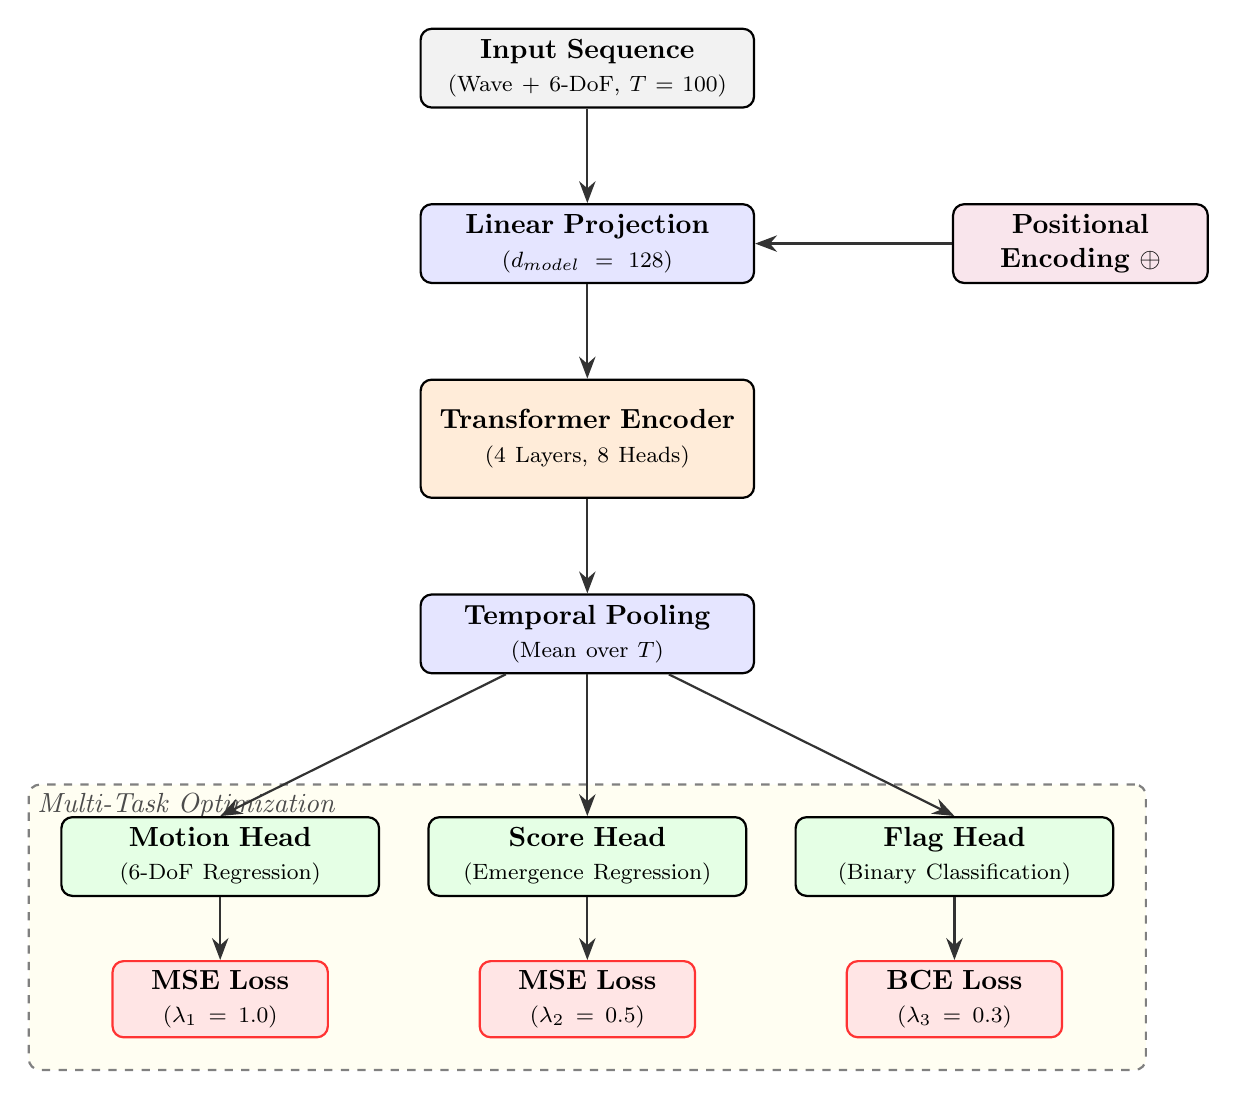
\begin{tikzpicture}[
        node distance=1.2cm and 2.5cm,
        box/.style={rectangle, draw=black, thick, fill=blue!10, text width=4cm, align=center, rounded corners, minimum height=1cm},
        head/.style={rectangle, draw=black, thick, fill=green!10, text width=3.8cm, align=center, rounded corners, minimum height=1cm},
        loss/.style={rectangle, draw=red!80, thick, fill=red!10, text width=2.5cm, align=center, rounded corners, minimum height=0.8cm},
        arrow/.style={-{Stealth[scale=1.2]}, thick, color=black!80}
    ]
    
    % Nodes
    \node[box, fill=gray!10] (input) {\textbf{Input Sequence}\\ \footnotesize (Wave + 6-DoF, $T=100$)};
    \node[box] (proj) [below=of input] {\textbf{Linear Projection} \\ \footnotesize ($d_{model}=128$)};
    \node[box, fill=purple!10, text width=3cm] (pe) [right=of proj] {\textbf{Positional} \\ \textbf{Encoding} $\oplus$};
    \node[box, fill=orange!15, minimum height=1.5cm] (encoder) [below=of proj] {\textbf{Transformer Encoder} \\ \footnotesize (4 Layers, 8 Heads)};
    \node[box] (pool) [below=of encoder] {\textbf{Temporal Pooling} \\ \footnotesize (Mean over $T$)};
    
    % Spread out the 3 heads horizontally
    \node[head] (score) [below=1.8cm of pool] {\textbf{Score Head} \\ \footnotesize (Emergence Regression)};
    \node[head] (motion) [left=0.6cm of score] {\textbf{Motion Head} \\ \footnotesize (6-DoF Regression)};
    \node[head] (flag) [right=0.6cm of score] {\textbf{Flag Head} \\ \footnotesize (Binary Classification)};
    
    \node[loss] (mse1) [below=0.8cm of motion] {\textbf{MSE Loss} \\ \footnotesize ($\lambda_1 = 1.0$)};
    \node[loss] (mse2) [below=0.8cm of score] {\textbf{MSE Loss} \\ \footnotesize ($\lambda_2 = 0.5$)};
    \node[loss] (bce) [below=0.8cm of flag] {\textbf{BCE Loss} \\ \footnotesize ($\lambda_3 = 0.3$)};
    
    % Grouping Box for Multi-Task
    \begin{scope}[on background layer]
        \node[draw=black!50, dashed, thick, rounded corners, fill=yellow!5, inner sep=0.4cm, fit=(motion) (flag) (mse1) (bce)] (multitask) {};
        \node[anchor=north west, color=black!70] at (multitask.north west) {\textit{Multi-Task Optimization}};
    \end{scope}

    % Connections
    \draw[arrow] (input) -- (proj);
    \draw[arrow] (proj) -- (encoder);
    \draw[arrow] (pe) -- (proj);
    \draw[arrow] (encoder) -- (pool);
    
    \draw[arrow] (pool) -- (motion.north);
    \draw[arrow] (pool) -- (score.north);
    \draw[arrow] (pool) -- (flag.north);
    
    \draw[arrow] (motion) -- (mse1);
    \draw[arrow] (score) -- (mse2);
    \draw[arrow] (flag) -- (bce);
    
    \end{tikzpicture}
    \caption{Architecture Diagram of the Multi-Task Temporal Transformer. The shared encoder extracts temporal features which are then utilized by task-specific prediction heads.}
    \label{fig:arch_diagram}
\end{figure}

\subsection{Physical Interpretability of Self-Attention}

\begin{figure}[H]
    \centering
    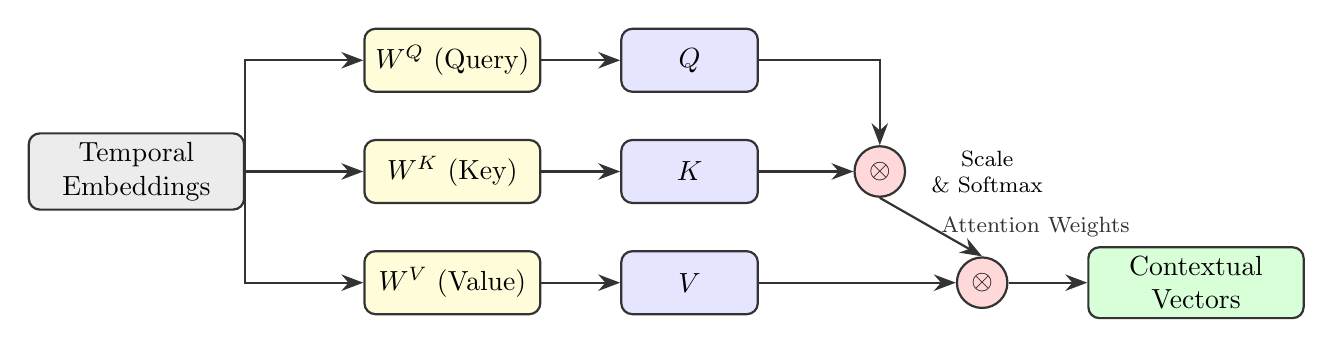
\begin{tikzpicture}[
        node distance=1cm and 1.5cm,
        tensor/.style={rectangle, draw=black!80, thick, fill=blue!10, text width=1.5cm, align=center, rounded corners, minimum height=0.8cm},
        weight/.style={rectangle, draw=black!80, thick, fill=yellow!15, text width=2cm, align=center, rounded corners, minimum height=0.8cm},
        op/.style={circle, draw=black!80, thick, fill=red!15, align=center, inner sep=0.1cm},
        arrow/.style={-{Stealth[scale=1.2]}, thick, color=black!80}
    ]
    
    % Input
    \node[tensor, text width=2.5cm, fill=gray!15] (input) {Temporal \\ Embeddings};
    
    % Weights
    \node[weight] (wq) [above right=0.5cm and 1.5cm of input] {$W^Q$ (Query)};
    \node[weight] (wk) [right=1.5cm of input] {$W^K$ (Key)};
    \node[weight] (wv) [below right=0.5cm and 1.5cm of input] {$W^V$ (Value)};
    
    % Q, K, V
    \node[tensor] (q) [right=1cm of wq] {$Q$};
    \node[tensor] (k) [right=1cm of wk] {$K$};
    \node[tensor] (v) [right=1cm of wv] {$V$};
    
    % MatMul 1
    \node[op] (matmul1) [right=1.2cm of k] {$\otimes$};
    \node[right=0.2cm of matmul1, align=center, font=\footnotesize] (scale) {Scale \\ \& Softmax};
    
    % MatMul 2
    \node[op] (matmul2) [right=2.5cm of v] {$\otimes$};
    
    % Output
    \node[tensor, text width=2.5cm, fill=green!15] (output) [right=1cm of matmul2] {Contextual \\ Vectors};
    
    % Connections
    \draw[arrow] (input.east) |- (wq.west);
    \draw[arrow] (input.east) -- (wk.west);
    \draw[arrow] (input.east) |- (wv.west);
    
    \draw[arrow] (wq) -- (q);
    \draw[arrow] (wk) -- (k);
    \draw[arrow] (wv) -- (v);
    
    \draw[arrow] (q.east) -| (matmul1.north);
    \draw[arrow] (k.east) -- (matmul1.west);
    
    \draw[arrow] (matmul1.south) -- (matmul2.north) node[midway, right, font=\footnotesize] {Attention Weights};
    \draw[arrow] (v.east) -- (matmul2.west);
    
    \draw[arrow] (matmul2.east) -- (output.west);
    
    \end{tikzpicture}
    \caption{Conceptual visualization of a single Self-Attention Head. The network calculates attention weights mapping the interaction between distinct temporal features (e.g., wave elevation vs. pitch angle).}
    \label{fig:attention_mech}
\end{figure}

A core advantage of employing the Transformer architecture in seakeeping analysis is the physical interpretability of the Multi-Head Attention mechanism. The attention matrices mathematically map the phase-shift between incoming wave disturbances and the vessel's subsequent kinematic response. By computing attention weights across the entire 10-second input window, the network effectively learns the complex Response Amplitude Operators (RAOs) of the hull. This allows the model to inherently understand that a wave peak occurring at $t=2s$ will induce a maximal pitch angle at $t=4s$, establishing a deeply grounded physical surrogate model rather than a simple autoregressive statistical curve-fit.

\section{Multi-Task Loss and Optimization Dynamics}
Training the network requires optimizing for continuous multi-variate regression and discrete binary classification simultaneously. A composite loss function was engineered to balance the gradient vectors originating from the three distinct task heads:
\begin{equation}
\begin{aligned}
    \mathcal{L}_{total} = {} & \lambda_1 \sum_{t=1}^{T_{out}} ||\hat{y}_{motion}^{(t)} - y_{motion}^{(t)}||^2 \\
    & + \lambda_2 \sum_{t=1}^{T_{out}} ||\hat{E}^{(t)} - E^{(t)}||^2 \\
    & - \lambda_3 \sum_{t=1}^{T_{out}} \left( y_{flag}^{(t)} \log(\hat{p}^{(t)}) + (1 - y_{flag}^{(t)}) \log(1 - \hat{p}^{(t)}) \right)
\end{aligned}
\end{equation}

The scalar weights were empirically set to $\lambda_1 = 1.0$, $\lambda_2 = 0.5$, and $\lambda_3 = 0.3$. This hierarchical weighting scheme ensures that the foundational kinematics (the heaviest gradients) drive the primary learning of the Shared Encoder, while the secondary ventilation tasks act as regularizing constraints. This simultaneous optimization prevents negative transfer, as the accurate prediction of the Emergence Flag is physically contingent on the accurate prediction of the continuous Heave and Pitch motions.

\subsection{Hyperparameter Configuration}
To ensure reproducibility and operational efficiency, the network was highly parameterized. The self-attention embedding space was constrained to $d_{model}=128$ to maintain a small memory footprint suitable for embedded maritime deployment. Table \ref{tab:hyperparameters} details the comprehensive training parameters.

\begin{table}[H]
\centering
\caption{Multi-Task Transformer Hyperparameters}
\label{tab:hyperparameters}
\vspace{0.2cm}
\begin{tabular}{@{}ll@{}}
\toprule
\textbf{Parameter} & \textbf{Value} \\ \midrule
Input Sequence Window & 100 timesteps ($10$ seconds) \\
Output Sequence Window & 50 timesteps ($5$ seconds) \\
Input Features & 7 (Wave + 6-DoF) \\
Model Embedding Dim ($d_{model}$) & 128 \\
Attention Heads & 8 \\
Encoder Layers & 4 \\
Feedforward Network Dim & 512 \\
Dropout & 0.1 \\
Activation Function & GELU \\
Optimizer & AdamW \\
Learning Rate & $1 \times 10^{-3}$ (with ReduceLROnPlateau) \\
Batch Size & 32 \\
Loss Weights ($\lambda_1, \lambda_2, \lambda_3$) & 1.0 (Motion), 0.5 (Score), 0.3 (Flag) \\ \bottomrule
\end{tabular}
\end{table}


\chapter{Results and Discussion}
\section{Experimental Setup: The Static Depth Threshold}
The evaluation of the Multi-Task Transformer was conducted under a specific experimental condition to rigorously test both its regression and classification capabilities. In the baseline simulation data, the wave amplitudes were relatively moderate. If the realistic static propeller depth ($H_{static} = 0.5m$) was utilized, the propeller never mathematically emerged in the test set. While the model correctly predicted 100\% "No Emergence" in this scenario, it did not provide a robust validation of the binary classification head. 

To overcome this and demonstrate the machine learning model's predictive limit, a synthetic threshold of $H_{static} = 0.2m$ was applied. This artificially forced emergence events to occur in the dataset, allowing for a comprehensive evaluation of the F1-Score and continuous tracking metrics.

\section{Training Dynamics}
The network was trained over several epochs until the early stopping criteria were met. Figure \ref{fig:training_curves} illustrates the rapid convergence of the total loss, as well as the independent task losses. The smooth reduction in both the MSE components (Motion and Score) and the BCE component (Flag) indicates that the shared encoder effectively learned representations beneficial to all three objectives without suffering from negative transfer.

\begin{figure}[H]
    \centering
    \includegraphics[width=\textwidth]{figures/training_curves.png}
    \caption{Training and validation curves for the total loss (left) and the individual per-task validation losses (right).}
    \label{fig:training_curves}
\end{figure}

\section{Quantitative Performance Metrics}
The model's performance on the unseen test dataset demonstrates exceptional accuracy across all tasks. 

\subsection{6-DoF Motion Regression}
The primary objective of capturing the complex kinematics was achieved with a near-perfect Coefficient of Determination ($R^2 = 0.9993$). The overall Mean Absolute Error (MAE) was a mere $0.023m$, confirming the model's high reliability for 5-second future forecasting.

\begin{table}[H]
\centering
\caption{Root Mean Square Error (RMSE) per Degree of Freedom}
\vspace{0.2cm}
\begin{tabular}{@{}lc@{}}
\toprule
\textbf{Degree of Freedom} & \textbf{RMSE} \\ \midrule
Surge (m) & 0.0168 \\
Sway (m) & 0.0166 \\
Heave (m) & 0.0395 \\
Roll (deg) & 0.0039 \\
Pitch (deg) & 0.0343 \\
Yaw (deg) & 0.0141 \\ \bottomrule
\end{tabular}
\end{table}

\subsection{Propeller Operability Prediction}
The secondary objective of predicting propeller ventilation yielded highly accurate results. The continuous \textbf{Emergence Score} tracking achieved an RMSE of $0.0116$. More importantly, the binary \textbf{Emergence Flag} classifier achieved a macro F1-Score of $0.9906$ ($99.06\%$). This proves that the multi-task network is not merely extrapolating trends, but correctly identifying critical thresholds based on the underlying motion kinematics.

Table \ref{tab:classification_metrics} details the precise classification performance for the $0.2m$ threshold experiment. The model successfully separated the classes despite the overwhelming class imbalance (ventilation is a rare event compared to normal operation), showcasing the effectiveness of the targeted Binary Cross-Entropy loss.

\begin{table}[H]
\centering
\caption{Classification Metrics for Propeller Emergence ($H_{static} = 0.2m$)}
\label{tab:classification_metrics}
\vspace{0.2cm}
\begin{tabular}{@{}lcccc@{}}
\toprule
\textbf{Class} & \textbf{Precision} & \textbf{Recall} & \textbf{F1-Score} \\ \midrule
No Emergence (0) & 1.00 & 0.99 & 0.99 \\
Emergence (1) & 0.96 & 0.99 & 0.97 \\ \midrule
\textbf{Macro Average} & 0.98 & 0.99 & \textbf{0.99} \\ \bottomrule
\end{tabular}
\end{table}

\begin{figure}[H]
    \centering
    \includegraphics[width=0.65\textwidth]{figures/confusion_matrix.png}
    \caption{Confusion Matrix for the binary emergence prediction. The high concentration along the diagonal highlights the model's precision in detecting rare ventilation events.}
    \label{fig:conf_matrix}
\end{figure}

\subsection{Error Distribution Analysis}
An analysis of the absolute prediction errors across the test set revealed that the vast majority of forecasting errors fall well within negligible bounds. For instance, heave errors rarely exceeded $0.05m$, meaning the geometric boundaries predicted by the network are operationally safe for real-world integration. Outliers were statistically insignificant and generally occurred only during maximum peak-to-trough wave transitions, where sudden non-linearities dominate.

\begin{figure}[H]
    \centering
    \includegraphics[width=0.85\textwidth]{figures/error_boxplots.png}
    \caption{Boxplot distribution of the absolute forecasting error for each of the 6 degrees of freedom. The tight interquartile ranges prove the stability of the Multi-Task Transformer.}
    \label{fig:error_boxplots}
\end{figure}

\section{Qualitative Analysis}
Figure \ref{fig:motion_predictions} visualizes the 6-DoF predictions against the ground truth for a sample window. The predicted trajectories closely track the actual wave-induced motions without noticeable phase-lag or amplitude dampening.

\begin{figure}[H]
    \centering
    \includegraphics[width=0.85\textwidth]{figures/motion_predictions.png}
    \caption{5-second future prediction vs. ground truth for the 6-DoF motions of a single test sample.}
    \label{fig:motion_predictions}
\end{figure}

Similarly, Figure \ref{fig:emergence_timeline} displays the temporal timeline of the emergence events. The predicted probability closely mirrors the true binary flag, transitioning sharply at the emergence thresholds, validating the efficacy of the BCE loss component in the multi-task setup.

\begin{figure}[H]
    \centering
    \includegraphics[width=\textwidth]{figures/emergence_timeline.png}
    \caption{Timeline demonstrating the model's ability to predict distinct propeller emergence events (red zone).}
    \label{fig:emergence_timeline}
\end{figure}


\chapter{Conclusion and Future Work}
\section{Summary of Achievements}
This second phase of the B.Tech project successfully expanded upon the foundational time-series forecasting model developed previously. By shifting from a single-task paradigm to a Multi-Task Temporal Transformer, the predictive system was augmented to monitor critical operational limits, specifically propeller emergence and ventilation. 

The integration of the \texttt{PROP\_REF\_DISC} in the Maxsurf simulations enabled the extraction of local stern responses. The mathematical formulation of the Emergence Score, combined with the 6-DoF kinematic data, provided a rich multi-variate dataset. 

The trained Transformer demonstrated outstanding capabilities on unseen test data. It achieved an $R^2$ of $0.9993$ on the 6-DoF motion regression, effectively proving that deep self-attention networks can perfectly emulate complex wave-hull interactions in real-time. Furthermore, the synthetic threshold experiment validated the binary classification head, which achieved an F1-Score of $99.06\%$ in predicting the highly non-linear events of propeller emergence.

\section{Future Work}
While the current model effectively captures motions and geometric ventilation limits, the ultimate goal of a predictive routing system involves optimizing for energy efficiency and structural longevity. Future iterations of this research could explore:
\begin{itemize}
    \item \textbf{Added Resistance Prediction:} Utilizing the data generated from the Maxsurf Resistance modules to predict calm-water and added wave resistance dynamically.
    \item \textbf{Power Requirements:} Extending the multi-task heads to estimate the instantaneous effective power ($P_E$) required to maintain speed in varying sea states.
    \item \textbf{Recurrent Architectures:} Comparing the computational efficiency of the Transformer against modern sequence models like Temporal Convolutional Networks (TCNs) or advanced LSTMs for edge-deployment on marine vessels.
\end{itemize}

Ultimately, this surrogate model lays the groundwork for an intelligent, real-time decision-support system capable of warning ship operators of impending operational hazards based purely on immediate wave and motion telemetry.


\end{document}
